\begin{figure}[p]
  \centering
  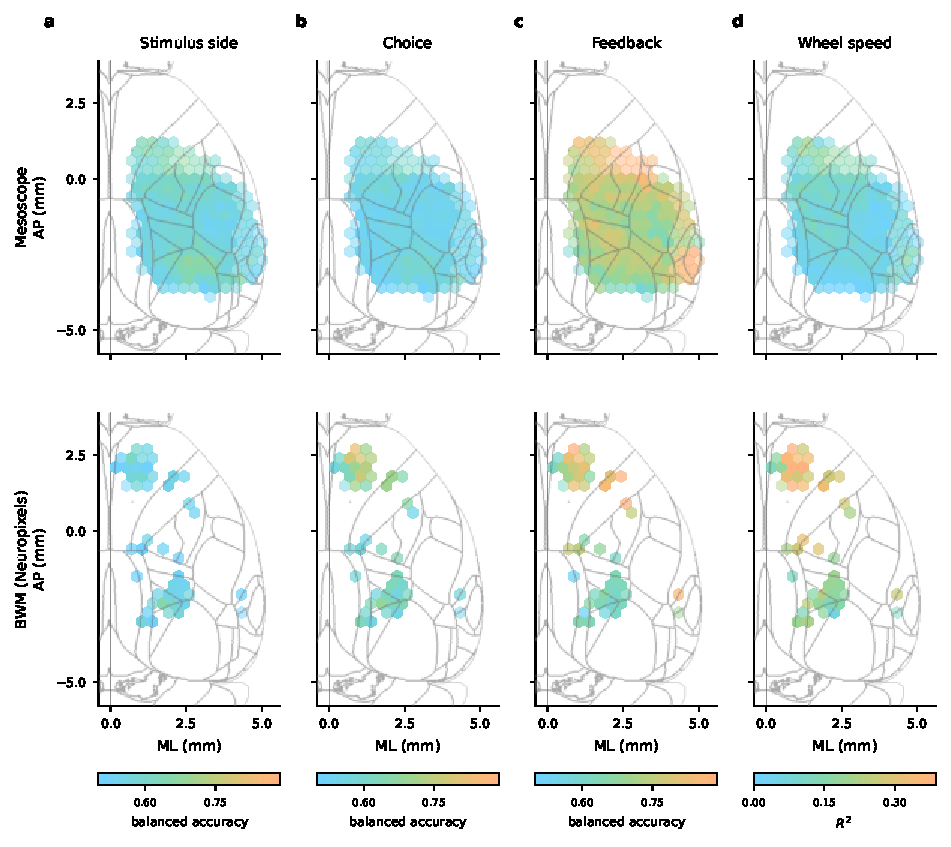
\includegraphics[width=7.00in,height=0.78\textheight,keepaspectratio]{si/si_strict_decoding_top_panels.pdf}
  \caption{Strict inclusion: only bins (0.4\,mm vertex to vertex, hemispheres folded) with $\geq$3 sessions from $\geq$2 animals, each session contributing $\geq$10 neurons. Isoluminant colour map; opacity encodes the number of animals (2: 50\,\%, 3: 75\,\%, $\geq$4: 100\,\%), so bins backed by few animals fade towards white. Mesoscope top row, BWM bottom row. Decoding from the 10 most selective neurons of the session in the bin, selected on the training trials of each cross-validation fold, averaged across sessions; otherwise as in the main decoding figures. The binary variables share one colour scale. \textbf{a} Stimulus side. \textbf{b} Choice. \textbf{c} Feedback. \textbf{d} Wheel speed ($R^2$).}
  \label{fig:si_strict_decoding_top}
\end{figure}
